%%%%%%%%%%%%%%%%%%%%%%%%%%%%%%%%%%%%%%%%%%%%%%%%%%%%%%%%%%%%%%%%%%%%%%
%%  Copyright by Wenliang Du.                                       %%
%%  This work is licensed under the Creative Commons                %%
%%  Attribution-NonCommercial-ShareAlike 4.0 International License. %%
%%  To view a copy of this license, visit                           %%
%%  http://creativecommons.org/licenses/by-nc-sa/4.0/.              %%
%%%%%%%%%%%%%%%%%%%%%%%%%%%%%%%%%%%%%%%%%%%%%%%%%%%%%%%%%%%%%%%%%%%%%%

\newcommand{\commonfolder}{../../common-files}
\newcommand{\webcommon}{../Web_Common}

\documentclass[11pt]{article}

\usepackage[most]{tcolorbox}
\usepackage{times}
\usepackage{epsf}
\usepackage{epsfig}
\usepackage{amsmath, alltt, amssymb, xspace}
\usepackage{wrapfig}
\usepackage{fancyhdr}
\usepackage{url}
\usepackage{verbatim}
\usepackage{fancyvrb}
\usepackage{adjustbox}
\usepackage{listings}
\usepackage{color}
\usepackage{subfigure}
\usepackage{cite}
\usepackage{sidecap}
\usepackage{pifont}
\usepackage{mdframed}
\usepackage{textcomp}
\usepackage{enumitem}
\usepackage{hyperref}


% Horizontal alignment
\topmargin      -0.50in  % distance to headers
\oddsidemargin  0.0in
\evensidemargin 0.0in
\textwidth      6.5in
\textheight     8.9in 

\newcommand{\todo}[1]{
\vspace{0.1in}
\fbox{\parbox{6in}{TODO: #1}}
\vspace{0.1in}
}


\newcommand{\unix}{{\tt Unix}\xspace}
\newcommand{\linux}{{\tt Linux}\xspace}
\newcommand{\minix}{{\tt Minix}\xspace}
\newcommand{\ubuntu}{{\tt Ubuntu}\xspace}
\newcommand{\setuid}{{\tt Set-UID}\xspace}
\newcommand{\openssl} {\texttt{openssl}}


\pagestyle{fancy}
\lhead{\bfseries SEED Labs}
\chead{}
\rhead{\small \thepage}
\lfoot{}
\cfoot{}
\rfoot{}


\definecolor{dkgreen}{rgb}{0,0.6,0}
\definecolor{gray}{rgb}{0.5,0.5,0.5}
\definecolor{mauve}{rgb}{0.58,0,0.82}
\definecolor{lightgray}{gray}{0.90}


\lstset{%
  frame=none,
  language=,
  backgroundcolor=\color{lightgray},
  aboveskip=3mm,
  belowskip=3mm,
  showstringspaces=false,
%  columns=flexible,
  basicstyle={\small\ttfamily},
  numbers=none,
  numberstyle=\tiny\color{gray},
  keywordstyle=\color{blue},
  commentstyle=\color{dkgreen},
  stringstyle=\color{mauve},
  breaklines=true,
  breakatwhitespace=true,
  tabsize=3,
  columns=fullflexible,
  keepspaces=true,
  escapeinside={(*@}{@*)}
}

\newcommand{\newnote}[1]{
\vspace{0.1in}
\noindent
\fbox{\parbox{1.0\textwidth}{\textbf{Note:} #1}}
%\vspace{0.1in}
}


%% Submission
\newcommand{\seedsubmission}{
Debe enviar un informe de laboratorio detallado, con capturas de pantalla, para describir lo que ha hecho y lo que ha observado.
También debe proporcionar una explicación a las observaciones que sean interesantes o sorprendentes.
Enumere también los fragmentos de código más importantes seguidos de una explicación. No recibirán créditos aquellos fragmentos de códigos que no sean explicados.}

%% Book
\newcommand{\seedbook}{\textit{Computer \& Internet Security: A Hands-on Approach}, 2nd
Edition, by Wenliang Du. Para más detalles \url{https://www.handsonsecurity.net}.\xspace}

%% Videos
\newcommand{\seedisvideo}{\textit{Internet Security: A Hands-on Approach},
by Wenliang Du. Para más detalles \url{https://www.handsonsecurity.net/video.html}.\xspace}

\newcommand{\seedcsvideo}{\textit{Computer Security: A Hands-on Approach},
by Wenliang Du. Para más detalles \url{https://www.handsonsecurity.net/video.html}.\xspace}

%% Lab Environment
\newcommand{\seedenvironment}{Este laboratorio ha sido testeado en nuestra imagen pre-compilada de una VM con Ubuntu 16.04, que puede ser descargada del sitio oficial de SEED.\xspace}

\newcommand{\seedenvironmentA}{Este laboratorio ha sido testeado en nuestra imagen pre-compilada de una VM con Ubuntu 16.04, que puede ser descargada del sitio oficial de SEED.\xspace}

\newcommand{\seedenvironmentB}{Este laboratorio ha sido testeado en nuestra imagen pre-compilada de una VM con Ubuntu 20.04, que puede ser descargada del sitio oficial de SEED .\xspace}

\newcommand{\seedenvironmentC}{Este laboratorio ha sido testeado en nuestra imagen pre-compilada de una VM con Ubuntu 20.04, que puede ser descargada del sitio oficial de SEED. Sin embargo, la mayoría de nuestros laboratorios pueden ser realizados en la nube para esto Ud. puede leer nuestra guía que explica como crear una VM de SEED en la nube.\xspace}

\newcommand{\seedenvironmentAB}{
Este laboratorio ha sido testeado en nuestras imagenes pre-compiladas de una VM con Ubuntu 16.04 y otra con Ubuntu 20.04, que pueden ser descargadas del sitio oficial de SEED.\xspace}

\newcommand{\nodependency}{Dado que utilizamos contenedores para configurar el entorno de laboratorio, este laboratorio no depende estrictamente de la VM de SEED. Puede hacer este laboratorio utilizando otras máquinas virtuales, máquinas físicas o máquinas virtuales en la nube.\xspace}

\newcommand{\adddns}{You do need to add the required IP address mapping to
the \texttt{/etc/hosts} file.\xspace}






\newcommand{\seedlabcopyright}[1]{
\vspace{0.1in}
\fbox{\parbox{6in}{\small Copyright \copyright\ {#1}\ \ by Wenliang Du.\\
      Este trabajo se encuentra bajo licencia Creative Commons.
       Attribution-NonCommercial-ShareAlike 4.0 International License.
       Si ud. remezcla, transforma y construye a partir de este material,
       Este aviso de derechos de autor debe dejarse intacto o reproducirse de una manera que sea razonable para el medio en el que se vuelve a publicar el trabajo.
       }}
\vspace{0.1in}
}






\lhead{\bfseries SEED Labs -- Laboratorio de CSRF}

\begin{document}

\begin{center}
{\LARGE Laboratorio de Cross-Site Request Forgery (CSRF)}
\vspace{0.1in}\\
{\Large (Web Application: {\tt Elgg})}
\end{center}

\seedlabcopyright{2006 - 2020}



% *******************************************
% SECTION
% ******************************************* 
\section{Descripción General}


El objetivo de este laboratorio, es ayudar a que los estudiantes entiendan el ataque de Cross-Site Request Forgery (CSRF). Un ataque de CSRF involucra un usuario víctima, un sitio de confianza y un sitio malicioso. La víctima tene una sesión válida en un sitio de confiana mientras que por otro lado visita un sitio malicioso que inyecta un request HTTP malicioso para ese sitio de confianza dentro de la sesión de la víctima.

En este laboratorio, los estudiantes usarán una aplicación web de red social para realizar ataques CSRF. La aplicación web se llama \texttt{Elgg} y ha sido instalada en nuestra Máquina Virtual. 
\texttt{Elgg} contiene contramedidas para prevenir ataques CSRF, pero las hemos desactivado para poder realizar los ataques.
Este laboratorio cubre los siguientes tópicos:


\begin{itemize}[noitemsep]
 \item Ataque de Cross-Site Request Forgery 
 \item Contramedidas para CSRF: Secret token y Same-site cookie
 \item Requests HTTP GET y POST
 \item JavaScript and Ajax
\end{itemize}


\paragraph{Lecturas.}
Para una cobertura más detallada en ataques CSRF puede consultar:

\begin{itemize}
\item Capítulo 10 del libro de SEED, \seedbook
\end{itemize}


\paragraph{Entorno de Laboratorio.} 
\seedenvironmentB 
\nodependency



% *******************************************
% SECTION
% *******************************************
\section{Configuración del Entorno de Laboratorio}

En este laboratorio, usaremos tres sitios web.
El primero será nuestro aplicativo web vulnerable Elgg y cuya URL es \url{www.seed-server.com}. El segundo será el sitio malicioso que va a ser usado para el ataque y cuya URL es \url{www.attacker32.com}. El tercero será el sitio usado para las tareas de defensa y su hostname es \url{www.example32.com}.
Usaremos contenedores para configurar el entorno de laboratorio.

% -------------------------------------------
% SUBSECTION
% -------------------------------------------
\subsection{Setup del Contenedor y sus Comandos}


%%%%%%%%%%%%%%%%%%%%%%%%%%%%%%%%%%%%%%%%%%%%
Para empezar a preparar el contenedor, deberá descargarse el archivo \texttt{Labsetup.zip} ubicado en el laboratorio correspondiente dentro del sitio web oficial y copiarlo dentro de la Máquina Virtual prevista por SEED. Una vez descargado deberá descomprimirlo y entrar dentro del directorio \texttt{Labsetup} donde encontrará el archivo \texttt{docker-compose.yml} que servirá para setear el entorno de laboratorio. Para una información más detallada sobre el archivo \texttt{Dockerfile} y otros archivos relacionados, puede encontrarla dentro del Manual de Usuario del laboratorio en uso, en el sitio web oficial de SEED.

Si esta es su primera experiencia haciendo el setup del laboratorio usando contenedores es recomendable que lea el manual anteriormente mencionado.

A continuación, se muestran los comandos más usados en Docker y Compose.
Debido a que estos comandos serán usados con mucha frecuencia, hemos creados un conjunto de alias para los mismos, ubicados en del archivo \texttt{.bashrc} dentro de la Máquina Virtual provista por SEED (Ubuntu 20.04)

\begin{lstlisting}
$ docker-compose build  # Build the container image
$ docker-compose up     # Start the container
$ docker-compose down   # Shut down the container

// Aliases for the Compose commands above
$ dcbuild       # Alias for: docker-compose build
$ dcup          # Alias for: docker-compose up
$ dcdown        # Alias for: docker-compose down
\end{lstlisting}


Dado que todos los contenedores estarán corriendo en un segundo plano. Necesitamos correr comandos para interactuar con los mismos, una de las operaciones fundamentales es obtener una shell en el contenedor. 
Para este propósito usaremos \texttt{"docker ps"} para encontrar el ID del contenedor deseado y ingresaremos \texttt{"docker exec"} para correr una shell en ese contenedor.
Hemos creado un alias para ello dentro del archivo \texttt{.bashrc}

\begin{lstlisting}
$ dockps        // Alias for: docker ps --format "{{.ID}}  {{.Names}}" 
$ docksh <id>   // Alias for: docker exec -it <id> /bin/bash

// The following example shows how to get a shell inside hostC
$ dockps
b1004832e275  hostA-10.9.0.5
0af4ea7a3e2e  hostB-10.9.0.6
9652715c8e0a  hostC-10.9.0.7

$ docksh 96
root@9652715c8e0a:/#  

// Note: If a docker command requires a container ID, you do not need to 
//       type the entire ID string. Typing the first few characters will 
//       be sufficient, as long as they are unique among all the containers. 
\end{lstlisting}

En caso de problemas configurando el entorno, por favor consulte la sección ``Common Problems'' en el manual ofrecido por SEED. 


%%%%%%%%%%%%%%%%%%%%%%%%%%%%%%%%%%%%%%%%%%%%


% -------------------------------------------
% SUBSECTION
% -------------------------------------------
\subsection{La Aplicación Web Elgg}

En este laboratorio usaremos una aplicación web de red social llamada Elgg.
Esta aplicación está instalada y configurada en las imágenes de nuestros contenedores. 
Usaremos dos contenedores, el primero será el encargado de correr el servidor web  (\texttt{10.9.0.5}) y el segundo será el encargado de correr el servidor de base de datos MySQL (\texttt{10.9.0.6}). 
Las direcciones IPs para ambos contenedores están hardcodeadas en múltiples lugares de los archivos de configuración del proyecto, por lo tanto se recomienda no cambiarlos en el archivo \texttt{docker-compose.yml}

\vspace{0.1in}
\paragraph{El Contenedor de Elgg.}
La aplicación web Elgg está hosteada usando un servidor web Apache.
La configuración del servidor está dentro del archivo \texttt{apache\_elgg.conf} dentro del directorio de la imagen Elgg.
Este archivo especifica la URL del sitio web y el directorio donde reside el código fuente de la aplicación web.

\begin{lstlisting}
<VirtualHost *:80>
     DocumentRoot /var/www/elgg
     ServerName   www.seed-server.com
     <Directory /var/www/elgg>
          Options FollowSymlinks
          AllowOverride All
          Require all granted
     </Directory>
</VirtualHost>
\end{lstlisting}

\paragraph{El Contenedor de Ataque.}
Usaremos otro contenedor para la máquina que será la atacante (\texttt{10.9.0.105}) y hosteará un sitio malicioso.
La configuración apache para este sitio web se muestra a continuación:

\begin{lstlisting}
<VirtualHost *:80>
     DocumentRoot /var/www/attacker
     ServerName   www.attacker32.com
</VirtualHost>
\end{lstlisting}
 
Debido a que necesitamos crear páginas web dentro de este contenedor, hemos montado un directorio en la Máquina Virtual Host (\texttt{Labsetup/attacker}) dentro del directorio del contenedor ubicado en \texttt{/var/www/attacker} que es el directorio usado por nuestro archivo configuración de Apache. A su vez las páginas web ubicadas dentro del directorio \texttt{attacker} en la Máquina Virtual, serán hosteadas en el sitio web del atacante. Hemos puesto un código genérico dentro de este directorio.

\paragraph{Configuración DNS.}
Accederemos a nuestro sitio Elgg, nuestro sitio malicioso y el sitio de defensa usando sus URLs.
Lo primero que hay que hacer es mapear los nombres de dominio del servidor web con sus IPs. Para ello deberá agregar las siguientes entradas en el archivo \texttt{/etc/hosts}.
Para poder modificar este archivo ud. debe contar con privilegios de root (usando \texttt{sudo}):

\begin{lstlisting}
10.9.0.5        www.seed-server.com
10.9.0.5        www.example32.com
10.9.0.105      www.attacker32.com
\end{lstlisting}


\vspace{-0.1in}
% MySQL database
%%%%%%%%%%%%%%%%%%%%%%%%%%%%%%%%%%%%

\paragraph{Base de Datos MySQL.}

Los contenedores suelen ser desechables, esto quiere decir que una vez que son destruidos, toda la información dentro de ellos se pierde por completo.
Para este laboratorio queremos que nuestra información quede persistida en la base de datos MySQL, por lo tanto no perderemos nuestro trabajo al apagar nuestro contenedor. Para lograr esto, hemos montado la carpeta \texttt{mysql\_data} en nuestra Máquina Host (dentro de la carpeta \texttt{Labsetup}, esta carpeta será creada después que el contenedor de MySQL sea creado y este corriendo) ubicada en el directorio \texttt{/var/lib/mysql} dentro del contenedor MySQL, en este directorio MySQL guardará todas las bases de datos.
Inclusive si el contenedor es destruido la información de la base de datos es conservada.
Si Ud. desea resetear la base de datos puede borrar la carpeta, usando el siguiente comando;
\begin{lstlisting}
$ sudo rm -rf mysql_data
\end{lstlisting}


%%%%%%%%%%%%%%%%%%%%%%%%%%%%%%%%%%%%


\vspace{-0.1in}
%%%%%%%%%%%%%%%%%%%%%%%%%%%%%%%%%%%%
%%%%%%%%%%%%%%%%%%%%%%%%%%%%%%%%%%%%%%%%%%%%%%%%%%%%%%%%%%%%%%%%%%%%%%
%%  Copyright by Wenliang Du.                                       %%
%%  This work is licensed under the Creative Commons                %%
%%  Attribution-NonCommercial-ShareAlike 4.0 International License. %%
%%  To view a copy of this license, visit                           %%
%%  http://creativecommons.org/licenses/by-nc-sa/4.0/.              %%
%%%%%%%%%%%%%%%%%%%%%%%%%%%%%%%%%%%%%%%%%%%%%%%%%%%%%%%%%%%%%%%%%%%%%%


\paragraph{Cuentas de Usuario.}
Hemos creado varias cuentas de usuario en el servidor de la aplicación {\tt Elgg}
Los usuarios y sus respectivos passwords son detalllados a continuación:


\begin{lstlisting}
----------------------------
UserName  | Password
----------------------------
admin     |  seedelgg
alice     |  seedalice 
boby      |  seedboby 
charlie   |  seedcharlie 
samy      |  seedsamy 
----------------------------
\end{lstlisting}





%%%%%%%%%%%%%%%%%%%%%%%%%%%%%%%%%%%%


% *******************************************
% SECTION
% ******************************************* 
\section{Tareas del Laboratorio: Ataques}


% -------------------------------------------
% SUBSECTION
% ------------------------------------------- 
\subsection{Tarea 1: Inspeccionando Request HTTP.}

Para realizar ataques CSRF, necesitamos capturar Requests HTTP.
En este laboratorio necesitaremos crear Requests HTTP. 
Para observar como luce un Request HTTP válido en Elgg, debemos ser capaces de capturar y analizar dichos requests.
Para este propósito usaremos un add-on para Firefox llamado \texttt{"HTTP Header Live"}. Antes de empezar el laboratorio, el estudiante debería estar familiarizado con esta herramienta.
Las instrucciones de como utilizarla están descriptas en esta sección (\S~\ref{web:sec:httpheaderlive}). En su informe de laboratorio, por favor identifique los parámetros usados en esos requests, si es que existen.


% -------------------------------------------
% SUBSECTION
% ------------------------------------------- 
\subsection{Tarea 2: Usando Request HTTP GET para el ataque CSRF}

In this task, we need two people in the Elgg social network: Alice
and Samy. Samy wants to become a friend to Alice, but Alice refuses to add 
him to her Elgg friend list. Samy decides to use the CSRF attack to
achieve his goal. He sends Alice an URL (via an email or a posting in 
Elgg); Alice, curious about it, clicks on the URL, which leads her to Samy's web site:    
\texttt{www.attacker32.com}. Pretend that you are Samy, describe how you
can construct the content of the web page, so as soon as Alice visits the
web page, Samy is added to the friend list of Alice (assuming Alice has an
active session with Elgg).


To add a friend to the victim, we need to identify what the legitimate 
Add-Friend HTTP request (a GET request) looks like. We can use 
the \texttt{"HTTP Header Live"} Tool to do the investigation. 
In this task, you are not allowed to
write JavaScript code to launch the CSRF attack. Your job is to make the
attack successful as soon as Alice visits the web page, without even making
any click on the page (hint: you can use the {\tt img} tag, which
automatically triggers an HTTP GET request).
 

Elgg has implemented a countermeasure to defend against 
CSRF attacks. In Add-Friend HTTP requests, you may notice that each 
request includes two weird-looking parameters, \texttt{\_\_elgg\_ts} and 
\texttt{\_\_elgg\_token}. These parameters are used by the countermeasure, so if they do not
contain correct values, the request will not be accepted by Elgg.   
We have disabled the countermeasure for this lab, so there is no need to include these two 
parameters in the forged requests. 


% -------------------------------------------
% SUBSECTION
% ------------------------------------------- 
\subsection{Tarea 3: Usando Request HTTP POST para el ataque CSRF}

After adding himself to Alice's friend list, Samy wants to do something more. He 
wants Alice to say ``Samy is my Hero'' in her profile, so everybody knows 
about that. Alice does not like Samy, let alone putting that statement 
in her profile. Samy plans to use a CSRF attack to achieve that goal. 
That is the purpose of this task. 


One way to do the attack is to post a message to Alice's Elgg account, hoping that 
Alice will click the URL inside the message. This URL will lead Alice to your (i.e., Samy's)
malicious web site \url{www.attacker32.com}, where you can launch the
CSRF attack. 

The objective of your attack is to modify the victim's profile. 
In particular, the attacker needs to forge a request 
to modify the profile information of the victim user of Elgg. 
Allowing users to modify their profiles is a feature of 
Elgg. If  users want to modify their profiles,
they go to the profile page of Elgg, fill out 
a form, and then submit the form---sending a POST request---to 
the server-side script {\tt /profile/edit.php}, which 
processes the request and does the profile modification.


The server-side script {\tt edit.php} accepts both GET and POST requests,
so you can use the same trick as that in Task 1 to achieve the attack.
However, in this task, you are required to use the POST request. 
Namely, attackers (you) need to forge an HTTP POST request from the victim's
browser, when the victim is visiting their malicious site. 
Attackers need to know the structure of such a request.
You can observe the
structure of the request, i.e.,  the parameters of the request, by making
some modifications to the profile and monitoring the request using
the \texttt{"HTTP Header Live"} tool. 
You may see something similar to
the following. Unlike HTTP {\tt GET} requests, which append 
parameters to the URL strings, the parameters of HTTP {\tt POST} requests are 
included in the HTTP message body (see the contents between the two 
\ding{80} symbols): 


\begin{lstlisting}
http://www.seed-server.com/action/profile/edit

POST /action/profile/edit HTTP/1.1
Host: www.seed-server.com
User-Agent: Mozilla/5.0 (X11; Ubuntu; Linux i686; rv:23.0) ...
Accept: text/html,application/xhtml+xml,application/xml;q=0.9,*/*;q=0.8
Accept-Language: en-US,en;q=0.5
Accept-Encoding: gzip, deflate
Referer: http://www.seed-server.com/profile/elgguser1/edit
Cookie: Elgg=p0dci8baqrl4i2ipv2mio3po05
Connection: keep-alive
Content-Type: application/x-www-form-urlencoded
Content-Length: 642
__elgg_token=fc98784a9fbd02b68682bbb0e75b428b&__elgg_ts=1403464813  (*@\ding{80}@*) 
&name=elgguser1&description=%3Cp%3Iamelgguser1%3C%2Fp%3E
&accesslevel%5Bdescription%5D=2&briefdescription= Iamelgguser1
&accesslevel%5Bbriefdescription%5D=2&location=US
......                                                              (*@\ding{80}@*)
\end{lstlisting}


After understanding the structure of the request, you need to 
be able to generate the request from your attacking web page
using JavaScript code. 
To help you write such a JavaScript program,  we provide a 
sample code in the following code fence. You can use this sample code to construct your malicious web site
for the CSRF attacks. This is only a sample code, and you need to modify it to 
make it work for your attack.


\begin{lstlisting}
<html>
<body>
<h1>This page forges an HTTP POST request.</h1>
<script type="text/javascript">

function forge_post()
{
    var fields;

    // The following are form entries need to be filled out by attackers. 
    // The entries are made hidden, so the victim won't be able to see them.
    fields += "<input type='hidden' name='name' value='****'>";
    fields += "<input type='hidden' name='briefdescription' value='****'>";
    fields += "<input type='hidden' name='accesslevel[briefdescription]' 
                                    value='2'>";                         (*@\ding{192}@*)
    fields += "<input type='hidden' name='guid' value='****'>";

    // Create a <form> element.
    var p = document.createElement("form");
	 
    // Construct the form
    p.action = "http://www.example.com";
    p.innerHTML = fields;
    p.method = "post";
	 
    // Append the form to the current page.
    document.body.appendChild(p);
	 
    // Submit the form
    p.submit();
}

	
// Invoke forge_post() after the page is loaded.
window.onload = function() { forge_post();}
</script>
</body>
</html>
\end{lstlisting}


In Line~\ding{192}, the value \texttt{2} sets the access level of a field to public. 
This is needed, otherwise, the access level will be set by default to private, so others cannot
see this field. It should be noted that when copy-and-pasting the above code
from a PDF file, the  single quote character in the program may become 
something else (but still looks like a single quote). That will cause 
syntax errors. Replacing all the single quote symbols with the one typed from 
your keyboard will fix those errors. 


\paragraph{Questions.}
In addition to describing your attack in full details, you also need to
answer the following questions in your report:

\begin{itemize}
   \item \textbf{Question 1}: The forged HTTP request needs Alice's user
   id (guid) to work properly. If Boby targets Alice specifically, before
   the attack, he can find ways to get Alice's user id. Boby does not know 
   Alice's Elgg password, so he cannot log into Alice's account to get
   the information. Please describe how Boby can solve this problem.

   
   \item \textbf{Question 2:} If Boby would like to launch the attack to
   anybody who visits his malicious web page. In this case, he does not
   know who is visiting the web page beforehand. Can he still launch the CSRF attack
   to modify the victim's Elgg profile? Please explain.
\end{itemize}





% *******************************************
% SECTION
% *******************************************
\section{Tareas de Laboratorio: Defensa} 

CSRF is not difficult to defend against. Initially, most applications
put a secret token in their pages, and by checking whether the token
is present in the request or not, they can tell whether a request
is a same-site request or a cross-site request. This is called
\textit{secret token} approach. 
More recently,
most browsers have implemented a mechanism called 
\textit{SameSite cookie}, which is intended to simplify the 
implementation of CSRF countermeasures. We will 
conduct experiments on both methods. 


% -------------------------------------------
% SUBSECTION
% ------------------------------------------- 
\subsection{Tarea 4: Activando las Contramedidas en Elgg} 

To defend against CSRF attacks, web applications can embed a secret token
in their pages. All the requests coming from these pages must carry this 
token, or they will be considered as a cross-site request, and will
not have the same privilege as the same-site requests. 
Attacker will not be able to get this secret token, so their requests
are easily identified as cross-site requests. 


Elgg uses this secret-token approach as its 
built-in countermeasures to defend against CSRF attacks. 
We have disabled the countermeasures to make the attack work. 
Elgg embeds two parameters
{\tt\_\_elgg\_ts} and {\tt\_\_elgg\_token} in the request.
The two parameters are added to the HTTP message body for the POST requests and to the URL
string for the HTTP GET requests. The server will validate them
before processing a request. 


\paragraph{Embedding secret token and timestamp to web pages.}
Elgg adds security token and timestamp to all the HTTP requests. 
The following HTML code is present in all the forms where user action is required. 
These are two hidden fields; when the form is submitted, these
two hidden parameters are added to the request:

\begin{lstlisting}
<input type = "hidden" name = "__elgg_ts" value = "" />
<input type = "hidden" name = "__elgg_token" value = "" />
\end{lstlisting}

Elgg also assign the values of the security token and timestamp to JavaScript variables, 
so they can be easily accessed by the JavaScript code on the same page.

\begin{lstlisting}
elgg.security.token.__elgg_ts;
elgg.security.token.__elgg_token;
\end{lstlisting}


The secret token and timestamp are added to Elgg's web pages by the 
\path{vendor/elgg/elgg/views/default/input/securitytoken.php} 
module. The code snippet below shows how they are dynamically 
added to web pages.

\begin{lstlisting}
$ts = time();
$token = elgg()->csrf->generateActionToken($ts);

echo elgg_view('input/hidden', ['name' => '__elgg_token', 'value' => $token]);
echo elgg_view('input/hidden', ['name' => '__elgg_ts', 'value' => $ts]);
\end{lstlisting}


\paragraph{Secret token generation.}
Elgg's security token is a hash value (md5 message digest) of the site 
secret value (retrieved from database),
timestamp, user session ID and random generated session string. 
The code below shows the secret token generation in Elgg 
(in \path{vendor/elgg/elgg/engine/classes/Elgg/Security/Csrf.php}).


\begin{lstlisting}
/**
 * Generate a token from a session token (specifying the user), 
 * the timestamp, and the site key.
 */
public function generateActionToken($timestamp, $session_token = '') {
  if (!$session_token) {
          $session_token = $this->session->get('__elgg_session');
          if (!$session_token) {
                  return false;
          }
  }

  return $this->hmac
          ->getHmac([(int) $timestamp, $session_token], 'md5')
          ->getToken();
}
\end{lstlisting}


\paragraph{Secret token validation.}
The elgg web application validates the generated token and timestamp to
defend against the CSRF attack.  Every user action calls the 
\texttt{validate} function inside \texttt{Csrf.php}, and this function validates the tokens.
If tokens are not present or invalid, the action will be denied and the
user will be redirected. In our setup, we added 
a \texttt{return} at the beginning of this function, essentially
disabling the validation.

\begin{lstlisting}
public function validate(Request $request) {
   (*@\textbf{return;}@*) // Added for SEED Labs (disabling the CSRF countermeasure)

   $token = $request->getParam('__elgg_token');
   $ts = $request->getParam('__elgg_ts');
   ... (code omitted) ...
}
\end{lstlisting}



\paragraph{Task: Turn on the countermeasure.}
To turn on the countermeasure, get into the Elgg container, 
go to the \path{/var/www/elgg/vendor/elgg/elgg/engine/classes/Elgg/Security} 
folder, remove the \texttt{return} statement from \texttt{Csrf.php}.
A simple editor called \texttt{nano} is available from inside the 
container.  After making the change, 
repeat the attack again, and see whether your attack will
be successful or not. 
Please point out the secret tokens in the captured HTTP requests.
Please explain why
the attacker cannot send these secret tokens in the CSRF attack; what
prevents them from finding out the secret tokens from the web page?   

\textbf{It should be noted (important)} that when we launch the edit-profile attack
while the countermeasure is enabled, the failed attempt will
cause the attacker's page to be reloaded, which will
trigger the forged POST request again. This will lead to another 
failed attempt, so the page will be reloaded again and 
another forged POST request will be sent out. This endless loop
will slow down your computer. Therefore, after verifying that 
the attack failed, kill the tab to stop the endless loop. 



% -------------------------------------------
% SUBSECTION
% -------------------------------------------
\subsection{Tarea 5: Experimentando con la Contramedida SameSite Cookie} 

Most browsers have now implemented a mechanism called SameSite cookie, 
which is a property associated with cookies. When sending out 
requests, browsers will check this property, and decide whether 
to attach the cookie in a cross-site request. A web application can
set a cookie as SameSite if it does not want the cookie to be 
attached to cross-site requests. For example, they can mark
the session ID cookie as SameSite, so no cross-site request
can use the session ID, and will therefore not be able to 
launch CSRF attacks. 


To help students get an idea on how the SameSite cookies can
help defend against CSTF attacks, we have created a website
called \url{www.example32.com} on one of the containers. Please 
visit the following URL (the hostname is already mapped 
to \texttt{10.9.0.5} in the \texttt{/etc/hosts} file; if you are 
not using the SEED VM, you should add this mapping to your machine): 

\begin{lstlisting}
URL: http://www.example32.com/
\end{lstlisting}

Once you have visited this website once, three cookies will be 
set on your browser, \texttt{cookie-normal}, \texttt{cookie-lax},
and \texttt{cookie-strict}. As indicated by the name,
the first cookie is just a normal one, the second and third cookies
are samesite cookies of two different types (\texttt{Lax} and \texttt{Strict}
types). We have designed two sets of experiments to see 
which cookies will be attached when you send an HTTP request
back to the server. Typically, all the cookies belonging to the server
will be attached, but this is not the case if a cookie is a samesite type. 


Please follow the links for the two experiments. Link A points to a page 
on \url{example32.com}, while Link B points to a page 
on \url{attacker32.com}. Both pages are identical (except for the background
color), and they both send three different types of requests to
\url{www.example32.com/showcookies.php}, which
simply displays the cookies sent by the browser. By looking 
at the display results, you can tell which cookies were sent 
by the browser. Please do the following: 


\begin{itemize}
\item Please describe what you see and explain why some cookies are 
not sent in certain scenarios. 
 
\item Based on your understanding, please describe how the SameSite
cookies can help a server detect whether a request 
is a cross-site or same-site request. 

\item Please describe how you would use
the SameSite cookie mechanism to help Elgg defend against CSRF attacks. 
You only need to describe general ideas, and there is no need to 
implement them. 
\end{itemize}


\paragraph{Bonus points.} Although it is not required, students
are encouraged to modify the Elgg application, so they
can use the samesite cookie mechanism to defend against
CSRF attacks. We recommend instructors to give bonus points 
to the students who can do this. Students should check with 
their instructors regarding the bonus points.


% -------------------------------------------
% SUBSECTION
% ------------------------------------------- 
\section{Guías}

%%%%%%%%%%%%%%%%%%%%%%%%%%%%%%%%%%%%%%%%
%%%%%%%%%%%%%%%%%%%%%%%%%%%%%%%%%%%%%%%%%%%%%%%%%%%%%%%%%%%%%%%%%%%%%%
%%  Copyright by Wenliang Du.                                       %%
%%  This work is licensed under the Creative Commons                %%
%%  Attribution-NonCommercial-ShareAlike 4.0 International License. %%
%%  To view a copy of this license, visit                           %%
%%  http://creativecommons.org/licenses/by-nc-sa/4.0/.              %%
%%%%%%%%%%%%%%%%%%%%%%%%%%%%%%%%%%%%%%%%%%%%%%%%%%%%%%%%%%%%%%%%%%%%%%

\newcommand{\devtoolFigs}{../Web_Common/Figs}


% -------------------------------------------
% SUBSECTION
% ------------------------------------------- 
\subsection{Usando \texttt{"HTTP Header Live"} para inspeccionar Headers HTTP}
\label{web:sec:httpheaderlive}

La versión de Firefox 60 de nuestra Máquina Virtual de Ubuntu 16.04 no soporta el plugin \texttt{LiveHTTPHeader}, que fue usado en nuestra Máquina Virtual de Ubuntu 12.04.
Dada esta situación, se usará \texttt{"HTTP Header Live"} como reemplazo.
Las instrucciones de como habilitar y usar este plugin se muestran en la figura Figure~\ref{web:fig:httpheader} solamente haga click en el ícono mosotrado en el marcador \ding{192}; aparecerá una barra lateral en la izquierda, asegúrese que \texttt{HTTP Header Live} este seleccionada en la posición mostrada en el marcador \ding{193}. Luego haga click en cualquier link dentro de la página, todas los Requests HTTP serán capturados y mostrados dentro de la barra lateral mostrada en el marcador  \ding{194}.
Si hace click en cualquiera Request HTTP, se abrirá un pop-up que mostrará el Request HTTP seleccionado. Desafortunadamente hay un bug en este plugin (que aún se encuentra en desarrollo); no se mostrará nada dentro de este pop-up al menos que ud. cambie el tamaño del pop-up (Al parecer el evento de re-drawing se ejecuta automáticamente cuando se abre el pop-up, pero cambiando su tamaño ocasiona que este evento sea disparado y en consecuencia se renderize el contenido en pantalla)


\begin{figure}[htb]
\begin{center}
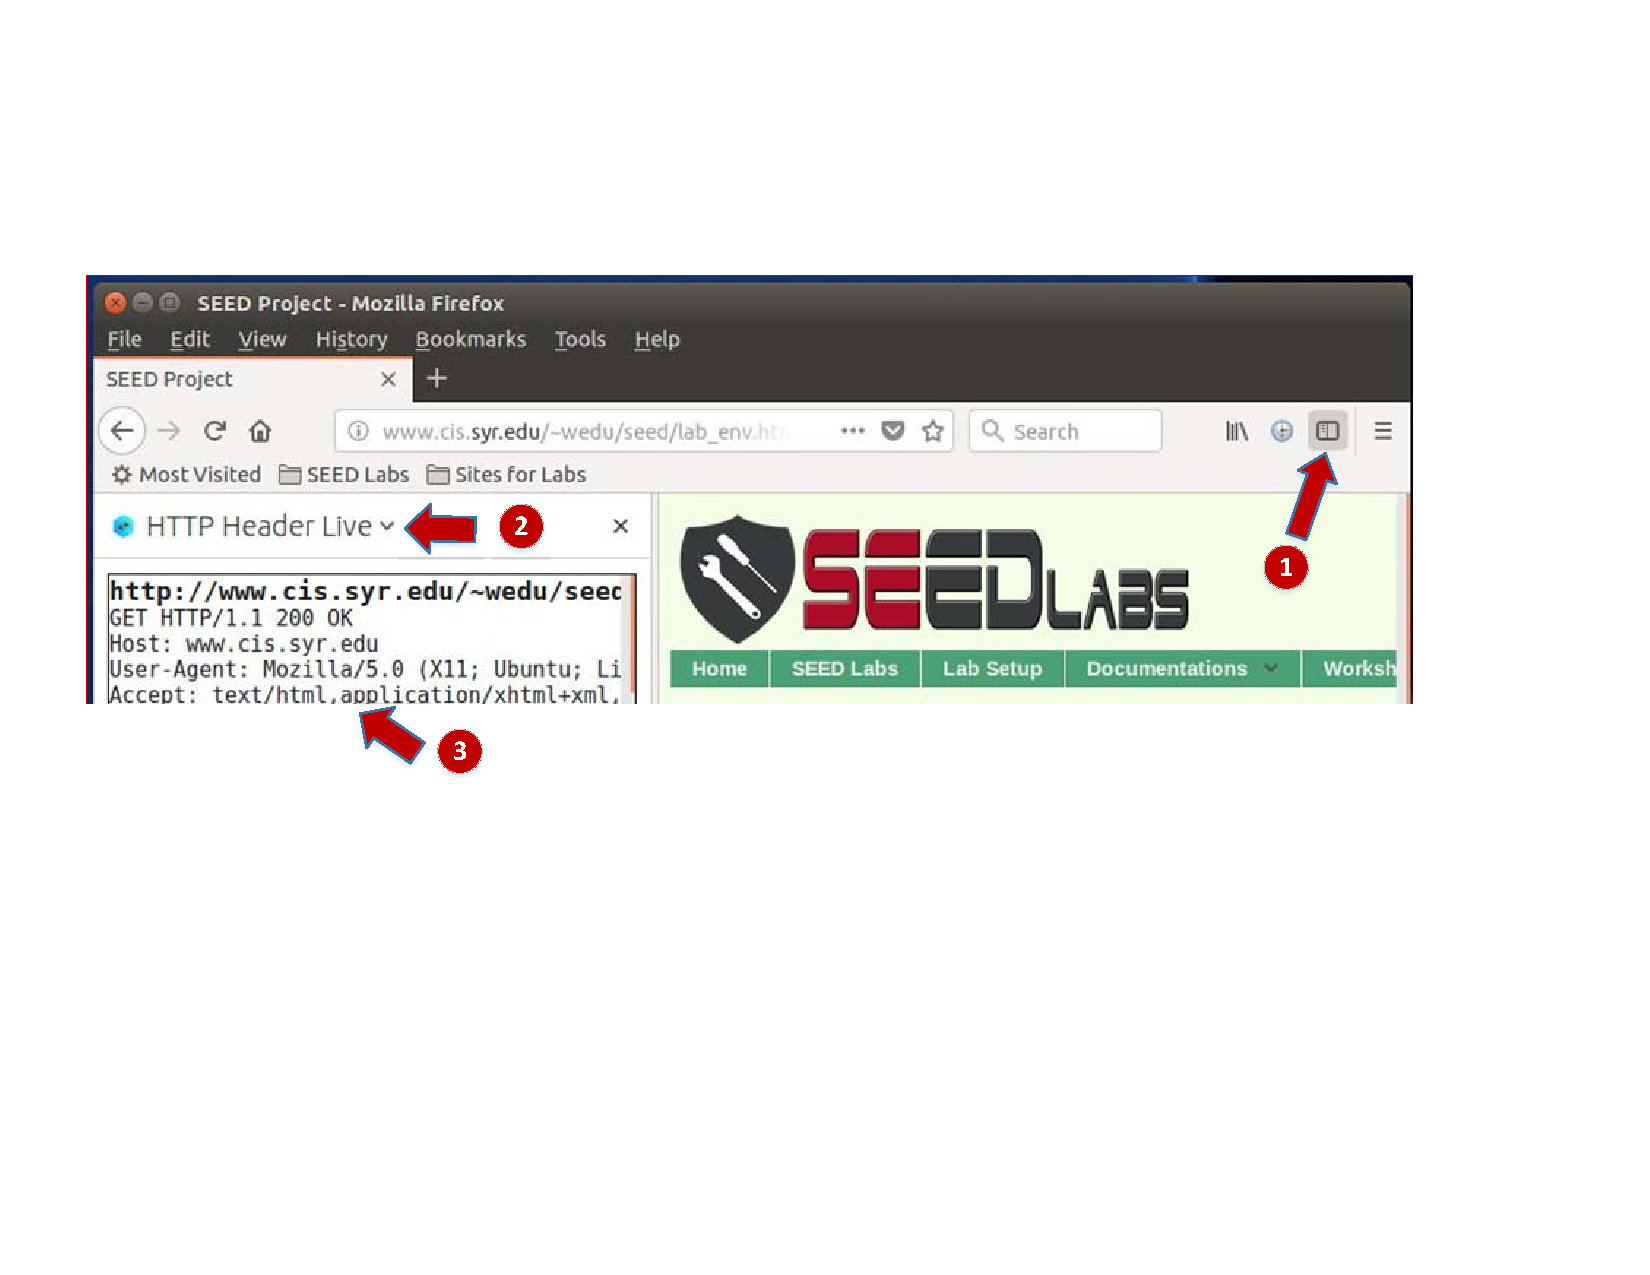
\includegraphics[width=0.85\textwidth]{\devtoolFigs/HTTPHeaderLive.pdf}
\end{center}
\caption{Hablitando el plugin HTTP Header Live}
\label{web:fig:httpheader}
\end{figure}




% -------------------------------------------
% SUBSECTION
% ------------------------------------------- 
\subsection{Usando Web Developer Tool para inspeccionar Headers HTTP}
\label{web:sec:web_dev_tools}

Existe otra herramienta provista por Firefox que puede ser muy útil para inspeccionoar Encabezados HTTP.
Esta herramienta es la Web Developer Network Tool. En esta sección, vamos a cubrir algunas de las features más importantes de esta herramienta.
La Web Developer Network Tool puede ser habilitada siguiendo estos pasos:

\begin{lstlisting}
Click Firefox's top right menu --> Web Developer --> Network
 or 
Click the "Tools" menu --> Web Developer --> Network 
\end{lstlisting}

Usaremos la página de login de Elgg como ejemplo.
La Figure~\ref{fig:webdevtools_01_request} muestra el Request HTTP POST que se envía al momento del login dentro de la Network Tool.

\begin{figure}[htb]
\begin{center}
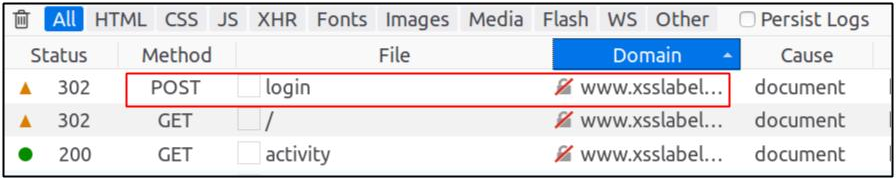
\includegraphics[width=0.8\textwidth]{\devtoolFigs/webdevtools_01_request.png}
\end{center}
\caption{Request HTTP en la Web Developer Network Tool}
\label{fig:webdevtools_01_request}
\end{figure}

Para más detalles del Request, podemos hacer click en un Request HTTP específico y se abrirán dos paneles con información detallada del mismo. (Ver Figure~\ \ref{fig:webdevtools_02_two_panes})

\begin{figure}[htb]
\begin{center}
	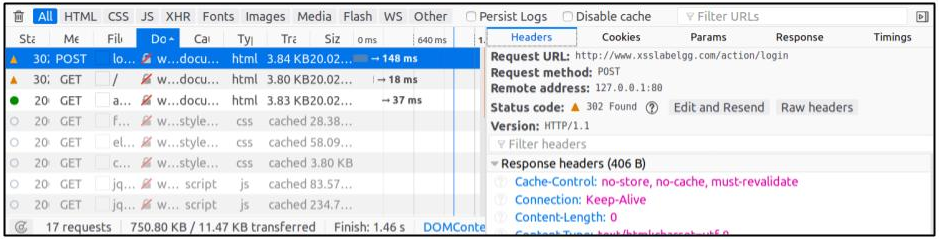
\includegraphics[width=0.95\textwidth]{\devtoolFigs/webdevtools_02_two_panes.png}
\end{center}
\caption{Request HTTP y Detalles del Request}
\label{fig:webdevtools_02_two_panes}
\end{figure}


Los detalles del Request seleccionado serán mostrados en el panel de la derecha.
La Figure~\ref{fig:webdevtools_03_post_headers} muestra los detalles del Request de Login en el Tab de 
\texttt{Headers} (Estos detalles incluyen el método del Request, la URL y la Cookie). En el panel derecho se pueden observar los Headers de la respuesta como también los del request.
Para chequear los parámetros involucrados en un request HTTP, podemos usar el tab \texttt{Params}. La Figure~\ref{fig:webdevtools_03_post_params} nos muestra los parámetros enviados en el request del login que se envía a Elgg, estos incluyen el \texttt{username} y el \texttt{password}. Esta herramienta puede ser usada para inspeccionar tanto Request HTTP GET como POST.

\begin{figure}[htb]
 \centering
 \subfigure[HTTP Request Headers]{
        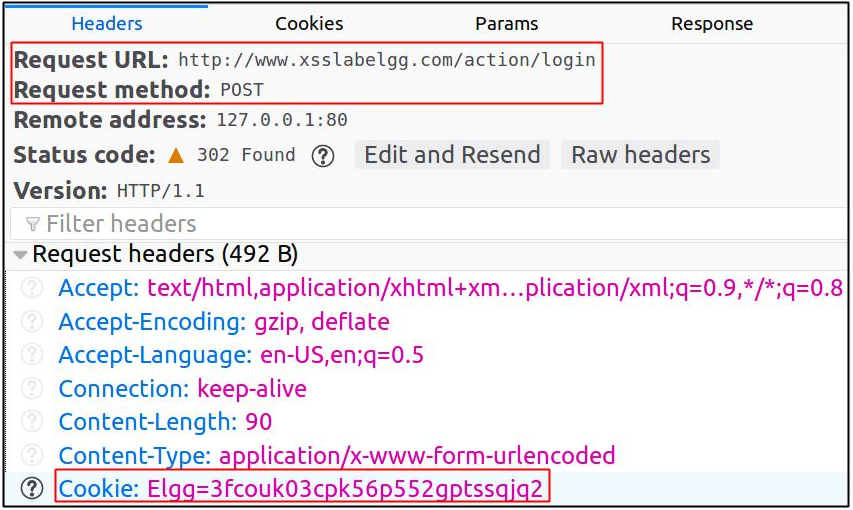
\includegraphics[width=0.6\textwidth]{\devtoolFigs/webdevtools_03-1.png}
        \label{fig:webdevtools_03_post_headers}
 }
 \subfigure[HTTP Request Parámetros]{
        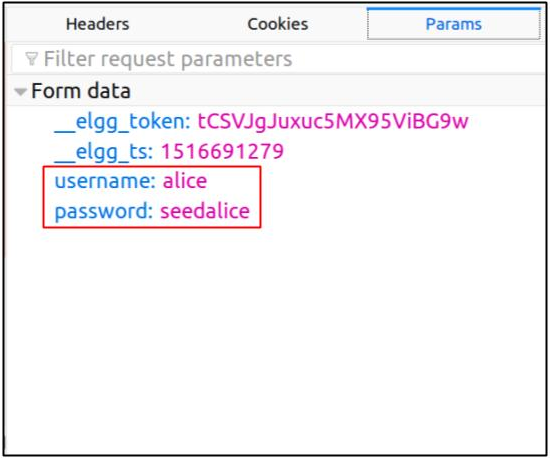
\includegraphics[width=0.35\textwidth]{\devtoolFigs/webdevtools_03-2.png}
        \label{fig:webdevtools_03_post_params}
 }
 \caption{HTTP Headers y Parámetros}
\end{figure}


\paragraph{Font Size.} El font size usado por defecto en la Web Developer Tool puede ser algo pequeño, para incrementar el tamaño de la fuente se debe hacer click en cualquier lugar de la ventana de la Network Tool y presionar en simultáneo las teclas \texttt{Ctrl} y \texttt{+} 



% -------------------------------------------
% SUBSECTION
% -------------------------------------------
\subsection{Debugueando JavaScript}
\label{web:sec:jsdebugging}

En muchas ocasiones vamos a necesitar debuguear nuestro código JavaScript. La developer tool de Firefox puede ayudarnos en esta tarea. Esta herramienta tiene la posibilidad de indicarnos el punto exacto en el código donde se produjo el error. A continuación se indica como habilitar el debugging en la Web Developer Tool:

\begin{lstlisting}
 Click the "Tools" menu --> Web Developer --> Web Console
 or use the Shift+Ctrl+K shortcut.
\end{lstlisting}

Una vez situados en la consola, se debe clickear en el tab {\tt JS}. Luego haga click en la flecha que apunta hacia abajo y asegúrese que al costado de {\tt Error} haya una tilde. Si también le interesa activar los mensajes de Warning en la coonsola seleccione {\tt Warnings}. Vea la Figure~\ref{devtool:fig:errocheckmark}.

\begin{figure}[htb]
\begin{center}
  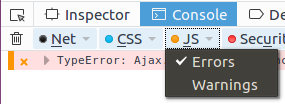
\includegraphics[width=0.4\textwidth]{\devtoolFigs/errorCheckMark.png}
\end{center}
\caption{Debugueando Código JavaScript (1)}
\label{devtool:fig:errocheckmark}
\end{figure}
 
Si hay errores en el código, se le mostrará un mensaje de error en la consola. Este mensaje indicará el número des línea que causó este error y estará ubicado en el extremo derecho del mensaje. Para ir al lugar exacto donde el código falló, deberá hacer click en el número de línea que es mostrado en el mensaje de error.
Vea la Figure~\ref{devtool:fig:console}.


\begin{figure}[htb]
\begin{center}
  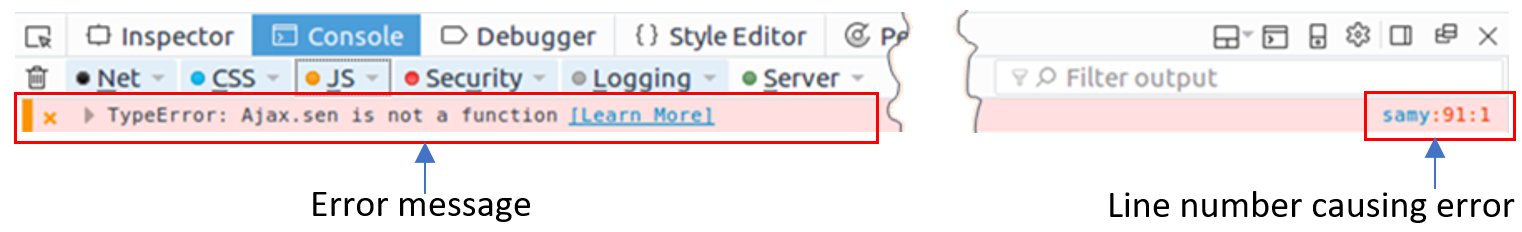
\includegraphics[width=1.0\textwidth]{\devtoolFigs/consoleError2.png}
\end{center}
\caption{Debugueando Código JavaScript (2)}
\label{devtool:fig:console}
\end{figure}
 




 

%%%%%%%%%%%%%%%%%%%%%%%%%%%%%%%%%%%%%%%%



% *******************************************
% SECTION
% ******************************************* 
\section{Informe de Laboratorio}


%%%%%%%%%%%%%%%%%%%%%%%%%%%%%%%%%%%%%%%%

Debe enviar un informe de laboratorio detallado, con capturas de pantalla, para describir lo que ha hecho y lo que ha observado.
También debe proporcionar una explicación a las observaciones que sean interesantes o sorprendentes.
Enumere también los fragmentos de código más importantes seguidos de una explicación. No recibirán créditos aquellos fragmentos de códigos que no sean explicados.
%%%%%%%%%%%%%%%%%%%%%%%%%%%%%%%%%%%%%%%%

% *******************************************
% SECTION
% *******************************************
\section*{Agradecimientos}

Este documento ha sido traducido al Español por Facundo Fontana



\end{document}



